\section{Apache Cassandra : qu’est-ce que c’est ?}
Apache Cassandra est un système de base de données distribuée très puissant, et particulièrement efficace pour prendre en charge de larges volumes d’enregistrements répartis sur de multiples serveurs. Initialement créé par Facebook, ce système est désormais open source.

Cette base de données peut être "scalée" facilement pour s’adapter à une augmentation soudaine de la demande. Il suffit pour cela de déployer des clusters Cassandra "multi-node". Par ailleurs, Cassandra est hautement disponible et présente l’avantage de ne pas avoir de point unique de défaillance.

\begin{figure}[h]
	\centering
    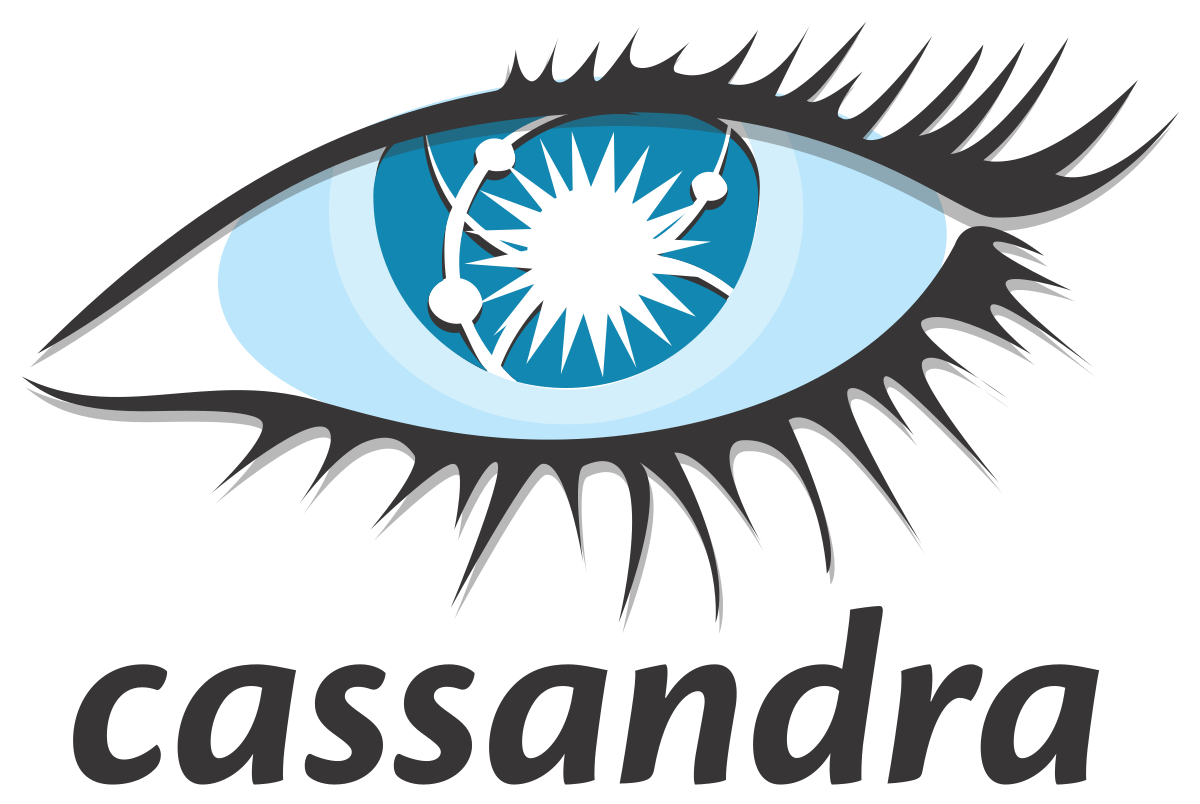
\includegraphics[scale=0.1]{img/part1/4.10}
    \caption{Logo CASSANDRA}
\end{figure}

\section{Historique:}
A l’origine, Apache Cassandra fut créé en interne par Facebook. L’objectif du géant américain était de développer un outil permettant à l’utilisateur du réseau social d’effectuer des recherches au sein de sa boîte de messages.

En juillet 2008, Facebook décide de rendre Cassandra open source. Un peu moins d’un an après, en mars 2009, Cassandra est accepté dans l’Apache Incubator. C’est en février 2010 que l’outil devient un projet Apache  » top-niveau « .
\\Depuis lors, Cassandra a beaucoup évolué. En 2021, la version actuelle est la 3.2.1. Cet outil est devenu extrêmement populaire face à l’essor du Big Data, à tel point que 40\% des entreprises du Fortune 100 l’utilisent. Outre Facebook, on peut aussi citer Netflix et Uber.